Linsen bestehen in der Regel aus einem optisch dichterem Medium als die umgebende Luft.
An den Grenzflächen wird das Licht gebrochen.
Zur Vereinfachung wird nun die gesamte Brechung der Linse, für achsennahe Strahlen, in der Mittelebene zusammengefasst.
Bei dickeren Linsen oder Linsensystemen ist dies nicht möglich und es müssen Hauptebenen eingeführt werden um die Brechung zu veranschaulichen.
Achsenferne Strahlen werden stärker gebrochen und führen so zu Abbildungsfehlern. Dieser Vorgang wird sphärische Abberration gennant.
Mit einer Blende können die achsenfernen Strahlen ausgeblendet werden. Die chromatische Abberration beschreibt die Brechung für unterschiedliche Wellenlängen,
so wird blaues Licht zum beispiel stärker gebrochen als rote Licht.
Es gibt zwei zu unterscheidende Linsenarten. Die konvexe Linse (Sammellinse, Abb. \ref{fig:sammellinse}) und die konkave Linse (Zerstreuungslinse, Abb. \ref{fig:streuungslinse}).
\begin{figure}[h!]
 \centering
 \begin{subfigure}{0.49\textwidth}
  \centering
  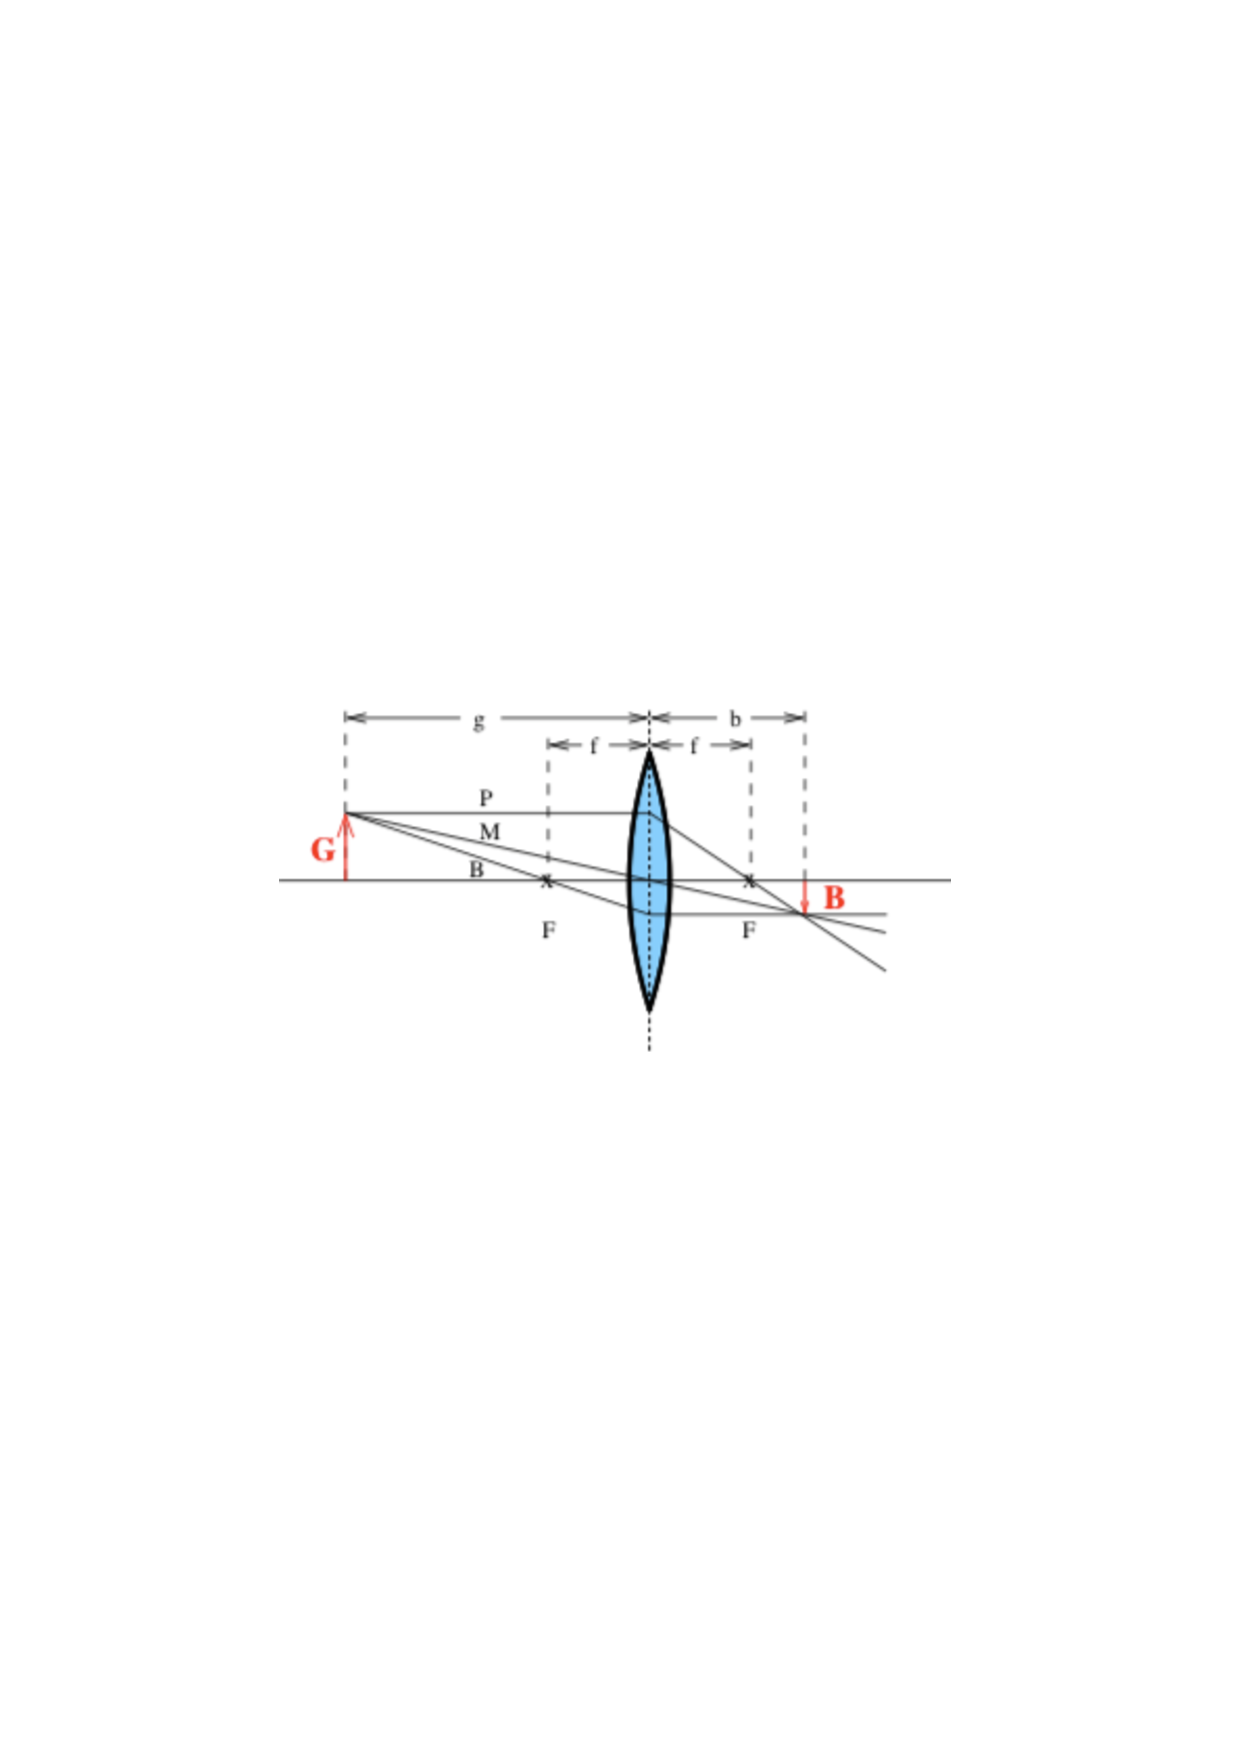
\includegraphics[width=0.9\textwidth]{sammellinse.pdf}
  \caption{Strahlengang einer Sammellinse \cite{1}}
  \label{fig:sammellinse}
 \end{subfigure}
 \begin{subfigure}{0.49\textwidth}
  \centering
  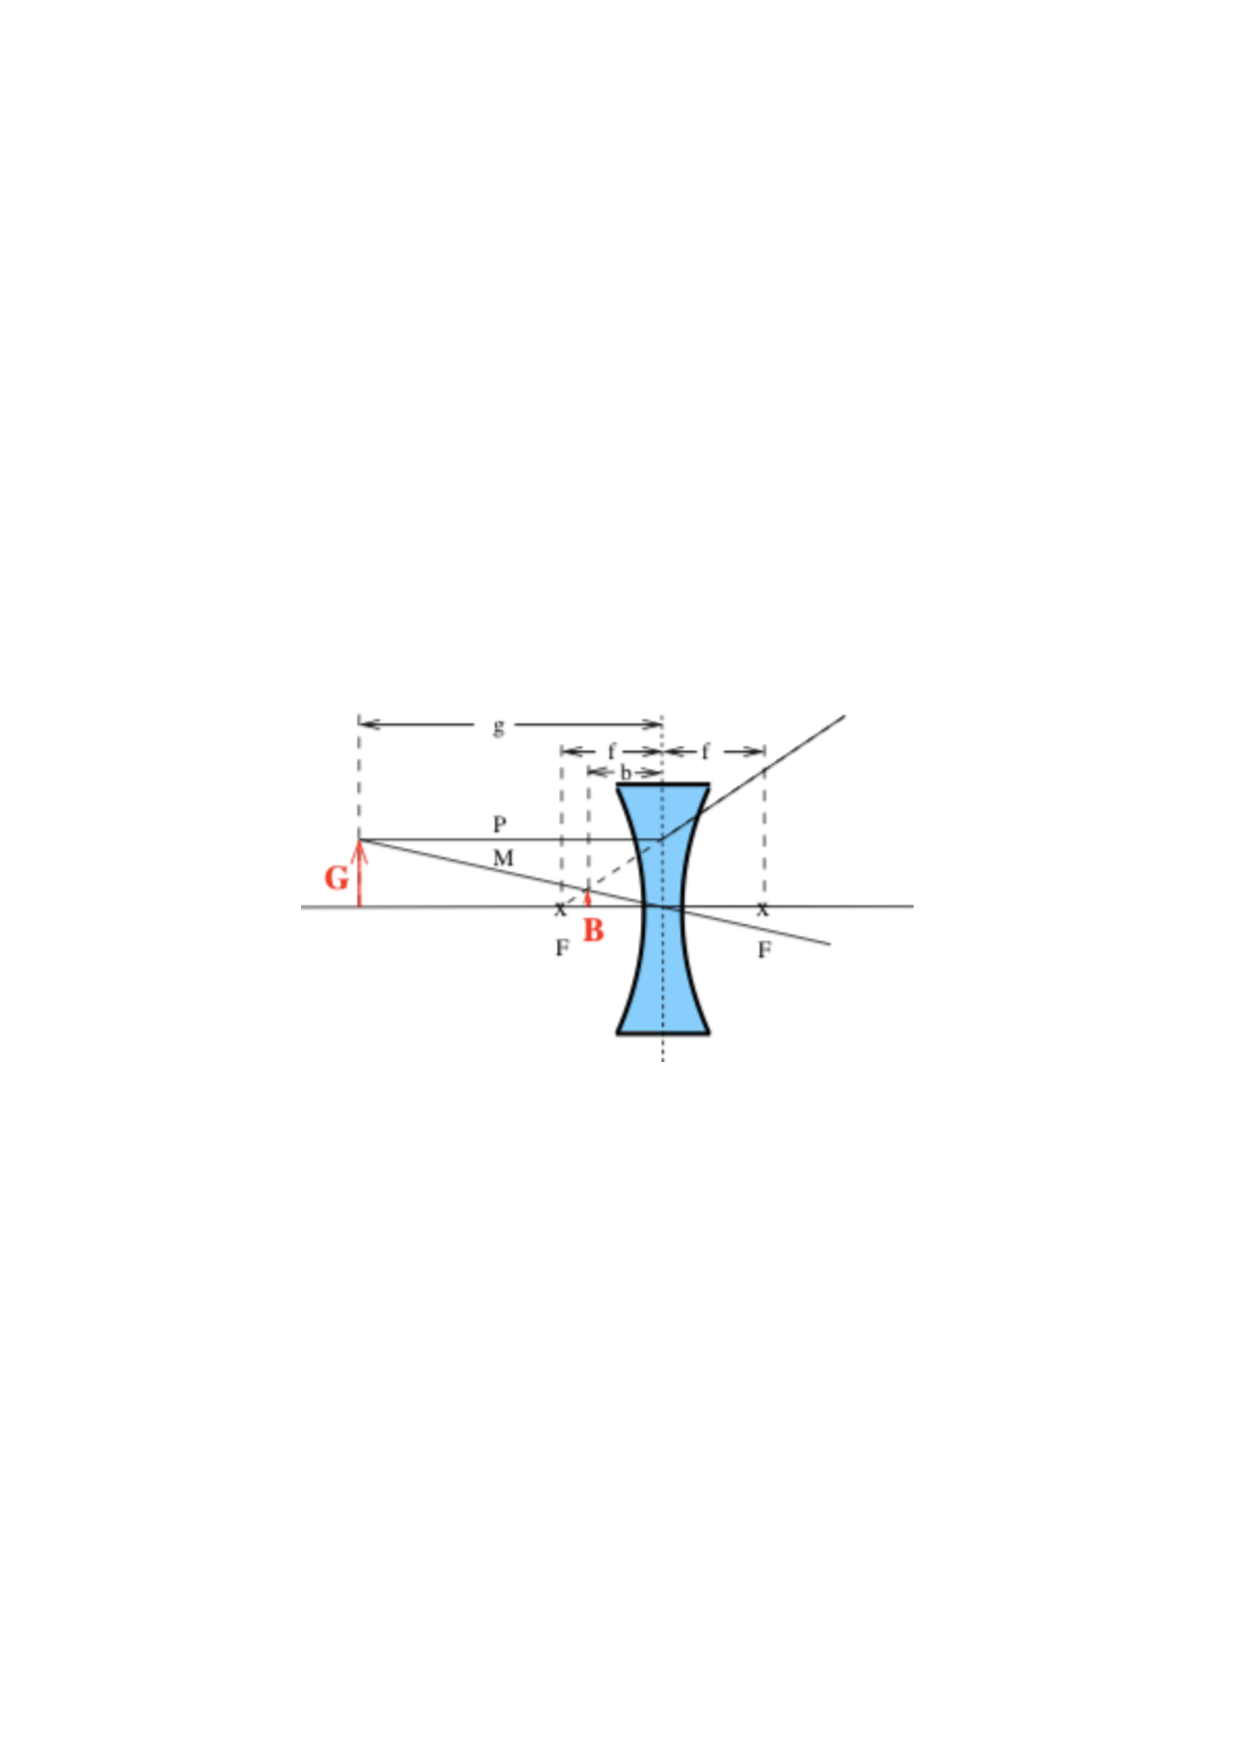
\includegraphics[width=0.9\textwidth]{streuungslinse.pdf}
  \caption{Strahlengang einer Zerstreuungslinse \cite{1}}
  \label{fig:streuungslinse}
 \end{subfigure}
 \caption{Verschiedene Linsen}
 \label{fig:linsen}
\end{figure}
\\Parallel einfallendes Licht wird von der Sammellinse im Brennpunkt F gebündelt.
Bei nicht-parallelem Licht wird dieses wie in der Abbildung \ref{fig:sammellinse} gebrochen.
Vom Gegenstand, der sich im Abstand $g$ vor der Linse befindet, werden zur Vereinfachung nur drei Strahlengänge betrachtet.
Der Strahl $P$ verläuft vom Gegenstand aus parallel zur optischen Achse und wird an der Mittelebene der Linse gebrochen und verläuft nun durch den Brennpunkt F, der sich in der Entfernung $f$ von der Mittelebene befindet.
Der Brennpunktstrahl B läuft zuerst durch den Brennpunkt F und wird durch die Brechung an der Linse zum parallelen Strahl.
Der Mittelstrahl M geht durch den Schnittpunkt von der optischen Achse und der Mittelebene. Der Mittelstrahl wird von der Linse nicht gebrochen.
Hinter der Linse gibt es einen Schnittpunkt in dem sich alle Strahlen kreuzen. An dieser Stelle, mit dem Abstand $b$, kann mit einem Schirm ein scharfes Bild B abgebildet werden.
\\Durch die Zerstreuungslinse wird das einfallende Licht gestreut. Der Strahl $P$ wird nach oben gebrochen.
Verlängert man den gebrochenen Strahl in Richtung des Gegensstandes $G$ fällt auf, dass dieser den Brennpunkt F vor der Linse schneidet.
Der Mittelpunktstrahl wird auch durch diese Linse nicht gebrochen. Sie besitzt jedoch eine Schnittstelle mit dem verlängerten gebrochenen Strahl.
Auf diese Weise entsteht ein virtuelles Bild $B$, im Abstand $b$, welches sich auf der Gegenstandsseite befindet.
\\Das Abbildungsgesetz folgt aus den Bildkonstruktionen.
\begin{align}
  V=\frac{B}{G}=\frac{b}{g}
  \label{eqn:maßstab}
\end{align}
$V$ beschreibt den Abbildungsmaßstab der sich für das Verhältnis von Bildgröße $B$ zu Gegenstandsgröße $G$ und Bildweite $b$ zu Gegenstandsweite $g$ gleich verhält.
Aus dem Abbildungsgesetz und der Bildkonstruktion lässt sich für dünne Linsen die Linsengleichung herleiten.
\begin{align}
  \frac{1}{f}=\frac{1}{b}+\frac{1}{g}
  \label{eqn:linse}
\end{align}
Die Brechkraft D wird in Dioptrie (dqt=$\SI{}{\frac{1}{f}}$) angegeben.
Bei einem System welches aus mehreren dünnen Linsen zusammengesetzt ist kann die Brechkraft $\text{D}_i$ aus den einzelnen Brechkräften zusammen gesetzt werden.
\begin{align*}
  \text{D}=\sum_{i}^{N}{\text{D}_i}\\
  \text{D}_i=\frac{1}{f}\SI{}{dpt}
\end{align*}
